\chapter{Improvement of the Calibration Process in ATLASCAR2}

Using sensors to recognize the environment is of most importance for vehicles to become fully autonomous. A car equipped with several sensors needs to know the position of each sensor so that the readings can be aligned and exact perception can be obtained. 

One of the main tasks for this dissertation is to be improve the extrinsic camera calibration process. Multi sensor calibration in ATLASCAR 2 is done using a ball as a target. One of the limitations of the approach in \cite{VieiradaSilva2016} is the use of filtering the image using HSV values to detect the ball.

While moving the ball around the sensors, a point cloud of ball centers is created for each sensor. These point clouds are aligned so that the estimate pose of each sensor can be obtained using an arbitrary sensor as reference.

\section{New Ball Detector Algorithm}

This section describes the progress introduced in the development of the ball detector.

\begin{figure}[htp]
	
	\centering
	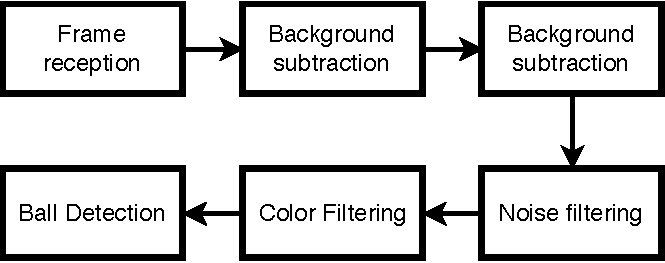
\includegraphics[width=0.8\textwidth]{capcalib/imgs/calib_implementation.pdf}
	
	\caption{New ball detection algorithm simplified diagram}
	\label{fig:ball_diagram}
	
\end{figure}

In figure \ref{fig:ball_diagram} a diagram showing the detection procedure is presented. As the frames are received, a background is selected to apply a background subtraction method. The noise from the resultant binary image is filtered and a color filtering method using the image color is applied to locate the ball by its color.

The ball detection upgrade begins by retrieving the video stream frames from the PointGrey camera. The image obtained was worked in a rosbag used for testing in order for the development to be made outside the ATLASCAR 2. The ball used in the tests is shown in figure \ref{fig:ball}. 

\begin{figure}[htp]
	
	\centering
	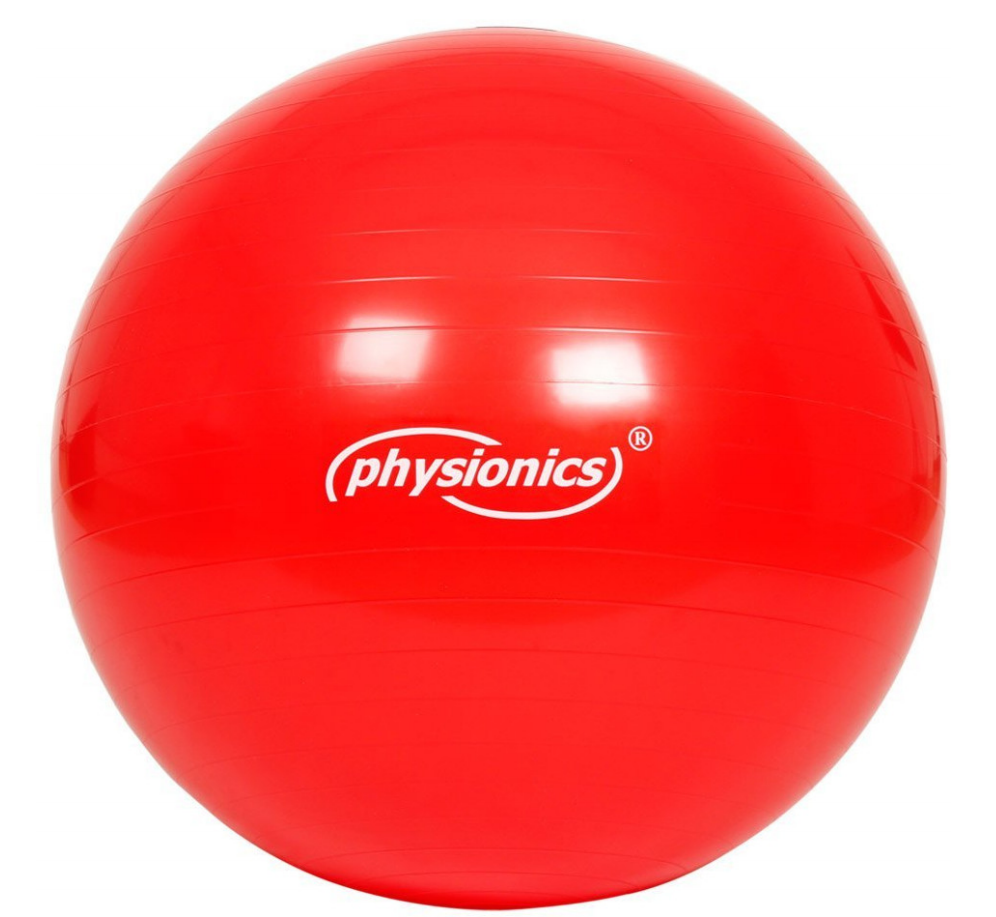
\includegraphics[width=0.4\textwidth]{capcalib/imgs/ball.png}
	
	\caption{Ball used for calibration testing}
	\label{fig:ball}
	
\end{figure}

To acquire the images, the ball detector node creates a subscriber to get messages from the camera topic. \gls{ros} subscribers take the message in the topic and send it to a callback function in order to it to be processed. After obtaining information from the camera's message, it is needed to convert the RGB values into the \gls{hsv} color space so that the image can be easily manipulated.

\subsection{Background Subtraction}

The first thing to do with the frames is to apply background subtraction. The vehicle is supposed to be still when the calibration process is being done, so the background subtraction is a good method to apply.

\begin{figure}[h!]
	
	\centering
	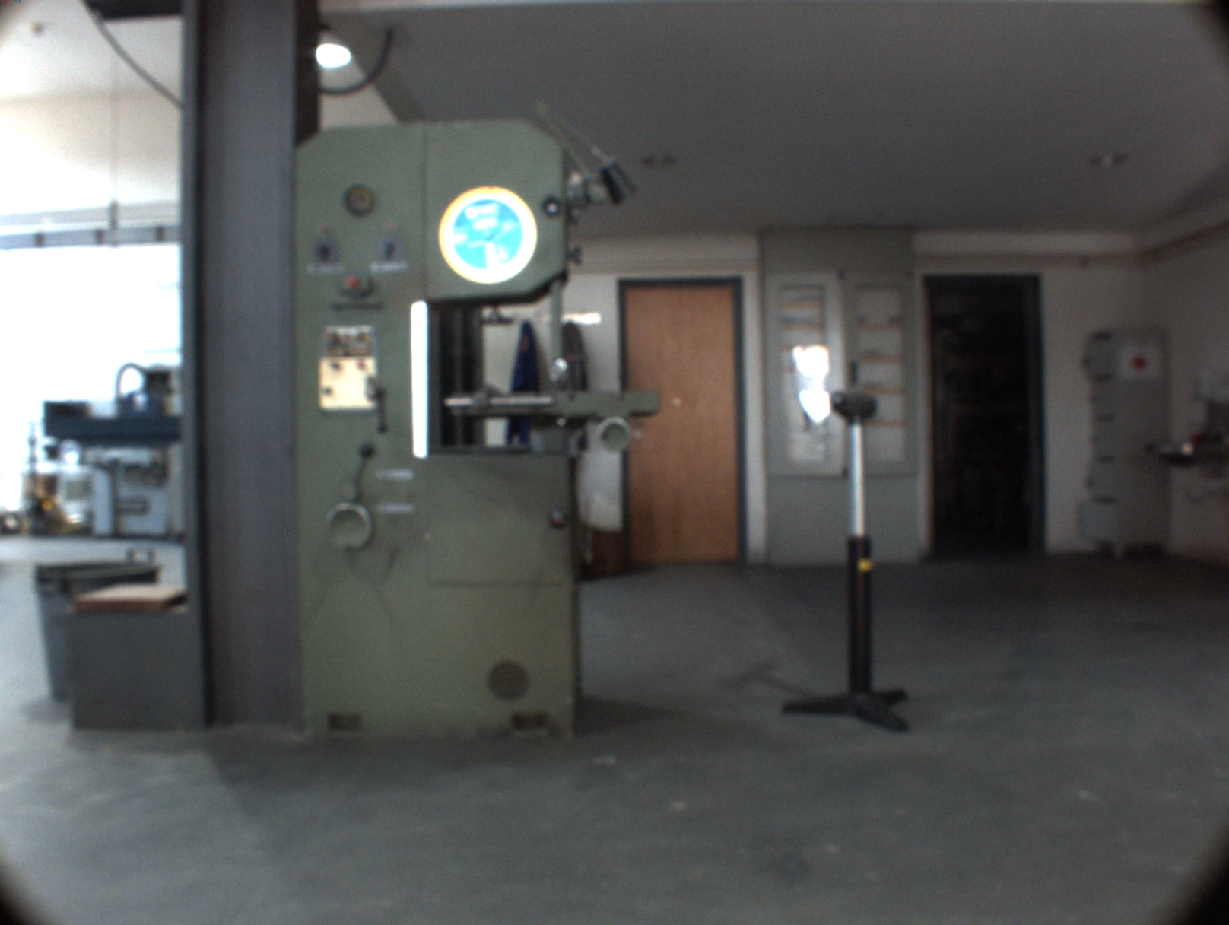
\includegraphics[width=0.65\textwidth]{capcalib/imgs/background.png}
	
	\caption{Background in test rosbag used for testing}
	\label{fig:background}
	
\end{figure}

When the capture starts, the first received frame will be the default background (see figure \ref{fig:background}). The background removal is a process used in many vision based applications with static cameras, in which a frame is captured and defined as the background of a sequence of images. Therefore, when an objects enters the scene (figure \ref{fig:balltest}), by subtracting the background with the actual frame it is possible to detect easily where the object is (\cite{OpenCV}).

\begin{figure}[htp]
	
	\centering
	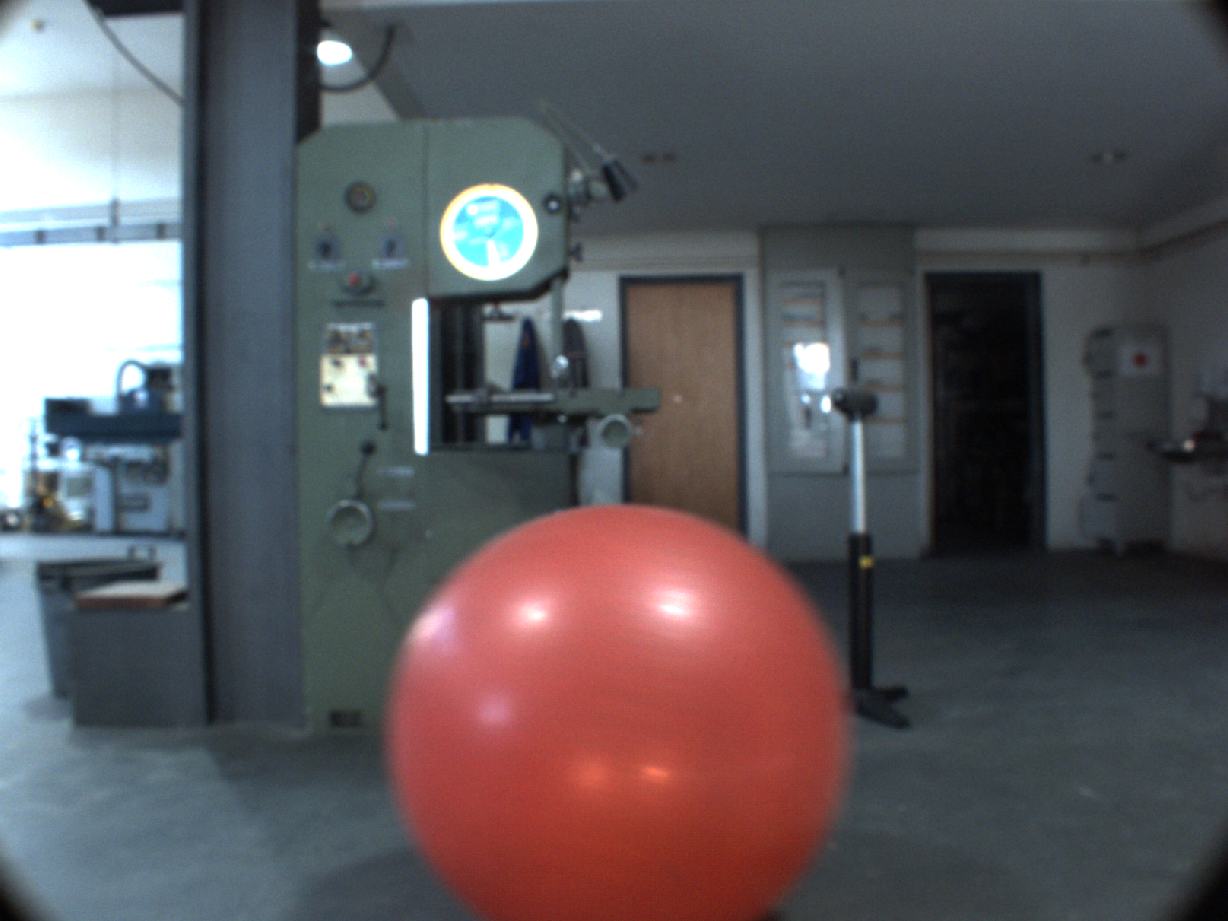
\includegraphics[width=0.8\textwidth]{capcalib/imgs/ball_test.png}
	
	\caption{Frame with ball rolling in front of the camera}
	\label{fig:balltest}
	
\end{figure}

In simple words, background subtraction extracts the foreground from the static background. Most times, the background is modified by applying Gaussian blur to it. When subtracting the foreground with the background, a value is obtained for each pixel.

In most cases the pixel values will not get to zero because of minor changes to the background (caused by shadows) which need to be ignored. In the resulting image a threshold is applied. If a pixel presents a value under the threshold, then it is set to zero (black), otherwise it is set to one (white). In the end, it is obtained a binary image containing some noise due to shadows or other lightning changes, and potentially an area with more concentrated white values where new objects appear. The result is a binary image as seen in figure \ref{fig:ballnoise}.


\begin{figure}[htp]
	
	\centering
	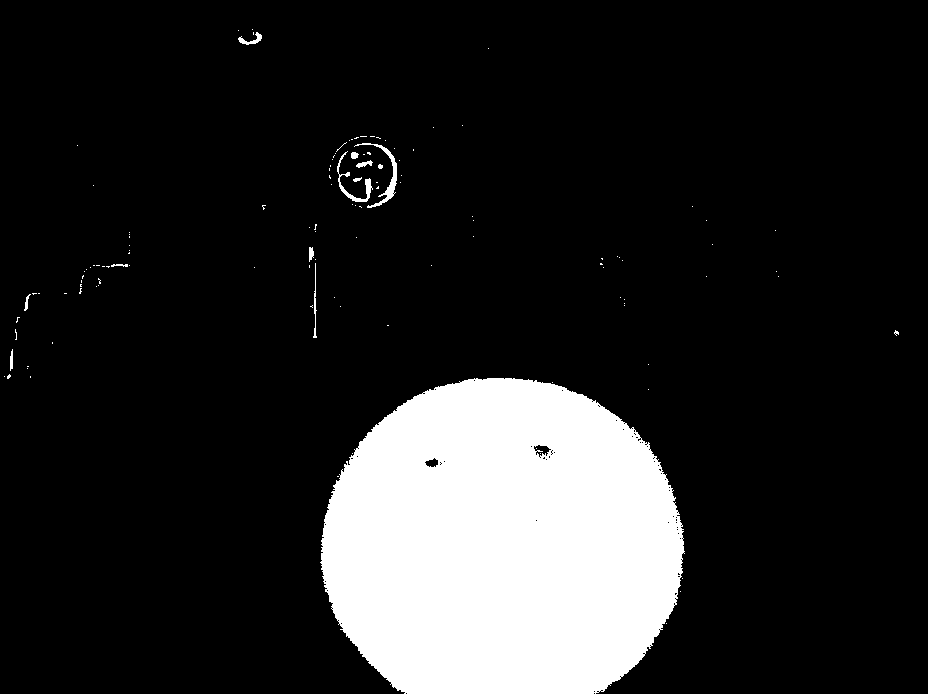
\includegraphics[width=0.8\textwidth]{capcalib/imgs/noise.png}
	
	\caption{Background subtraction result with noise}
	\label{fig:ballnoise}
	
\end{figure}

\subsection{Noise Filtering}

After the background removal technique is applied, the resulting image may possibly contain some noise. Some pixels may be left white in the background due to lightning changes when the ball passes in front of the camera. These white pixels are noise and must be removed.

An erosion algorithm is implemented where for each pixel the neighbor pixels are counted. The image is processed left-to-right, top-to-bottom, so the matrix corresponding to the frame is iterated throughout its lines. A counter is added to check if the previous pixels contained white pixels (with value of 1). 

As the kernel is scanned over the image, the algorithm computes the minimal pixel value overlapped by the kernel and replaces the image pixel under the anchor point with that minimal value (\cite{OpenCV2.4.13.6documentation}). The result is the image in figure \ref{fig:balldetect}.

\subsection{Color Filtering}

After the noise filtering, the ball stands out in the image. The next step is to separate the ball using color filtering. This step is necessary to make the detection usable when a person appears in the image to displace the ball. This way, the person will not appear in the resulting image.

The selected color by default is red. To set the ball color, the user needs to click in the ball to capture its hue. A mouse event is triggered and an handler function is called. The handler localizes the mouse click and retrieves the RGB values of the pixel in those coordinates. These values are converted to a hue value of the \gls{hsv} color space. The selected hue is the color used to filter the ball from the rest of the image. By applying certain thresholds it is possible to define an interval of color. The image will then be filtered by an interval centered in that hue value and the ball is now filtered from the rest of the image. 


\subsection{Bounding Box}

A bounding box is drawn around the ball if there is a number of white pixels bigger than a predefined threshold. To do this, the image is iterated like in this erosion phase, left-to-right and top-to-bottom. The algorithm saves the coordinates of all white pixels. An average $x$ and $y$ are calculated, finding the ball center in the image. The size of the bounding box is given by how much white is in an specific area. Supposing there is a possibility of a white pixel to appear as noise, that pixel will have low weight in the algorithm considering that the pixels around it are black. Therefore, white pixels gathered in a larger area have greater weight. Hence, the width and height of the bounding box are given by the maximum distance between the pixels with higher weight.


\begin{figure}[htp]
	
	\centering
	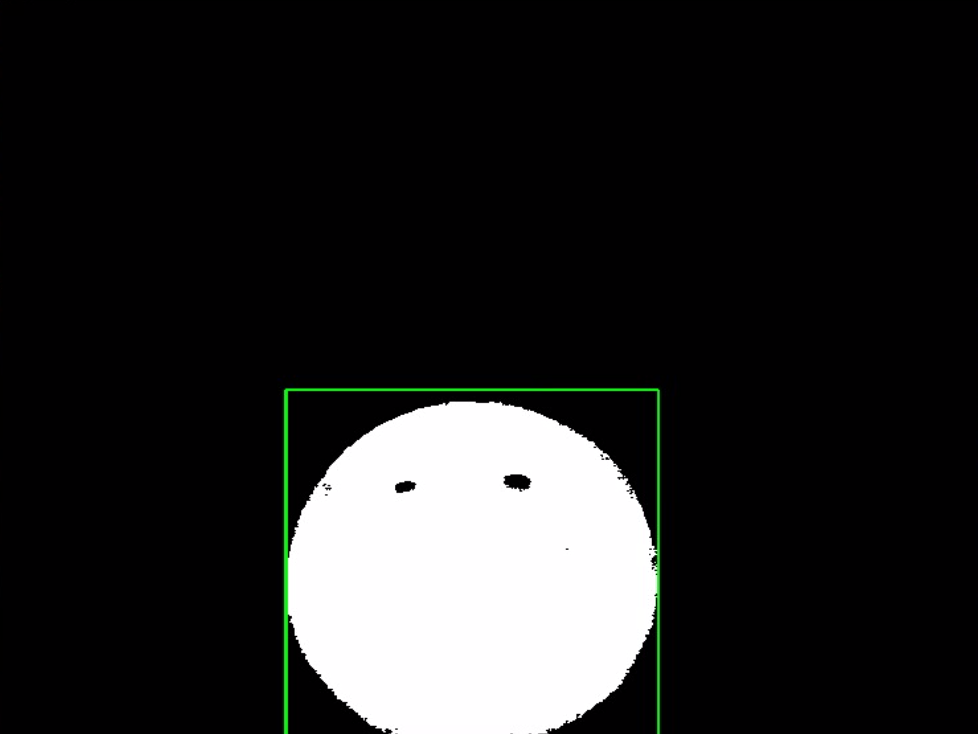
\includegraphics[width=0.5\textwidth]{capcalib/imgs/ball_detect.png}
	
	\caption{Ball detected with bounding box}
	\label{fig:balldetect}
	
\end{figure}

\section{Modifying the calibration package}

The calibration package used to calibrate the several sensors in ALTASCAR 2 uses multiple nodes, one for each kind of sensor. The camera node in the package is called \texttt{point\_grey\_camera} and it uses the source file \texttt{point\_grey\_camera.cpp}. This file was modified in order to add the implemented features into the calibration package. 

The \texttt{point\_grey\_camera} node receives the camera image by subscribing to the camera topic with \gls{ros}. The camera sends images in a \gls{ros} message format to be interpreted and processed by a callback function. The image processing algorithm follows the steps explained in the previous section. After performing the ball detection, the center of the bounding box matching the center of the ball is retrieved. The ball center is published into the calibration package main node \texttt{calibration\_gui}.

The radius of the ball is passed as an argument so it is possible to calculate the distance from the camera to it. The centroids are obtained with a method based on the circle radius and they are published as \texttt{PointStamped} \gls{ros} points to be presented in the calibration \gls{gui}. 















 

